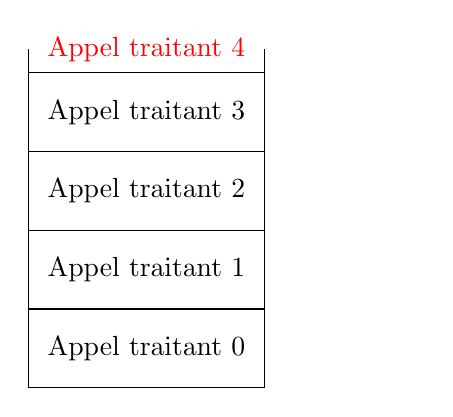
\begin{tikzpicture}
    \draw (0, 4.3) to (0, 0)
                 to (3, 0)
                 to (3, 4.3);
    \uncover<18->{\draw (0, 1) to (3, 1);
                 \node at (1.5, 0.5) {Appel traitant 0};}
    \uncover<19->{\draw (0, 2) to (3, 2);
                 \node at (1.5, 1.5) {Appel traitant 1};}
    \uncover<20->{\draw (0, 3) to (3, 3);
                 \node at (1.5, 2.5) {Appel traitant 2};}
    \uncover<21->{\draw (0, 4) to (3, 4);
                 \node at (1.5, 3.5) {Appel traitant 3};}
    \uncover<22->{\node[red] at (1.5, 4.3) {Appel traitant 4};}

    \node at (4, 0.5) {\phantom{Résultat~: 6}};
\end{tikzpicture}
